\documentclass[UTF8]{ctexart}
\usepackage{amsmath}
\usepackage{amssymb}
\usepackage{booktabs}
\usepackage{background}
\usepackage{caption,subcaption}
\usepackage{enumitem}
\usepackage{fancyhdr}
\usepackage{float}
\usepackage{fontspec}
%\usepackage{fourier}
\usepackage{geometry}
\usepackage{hyperref}
\usepackage{imakeidx}
\usepackage{listings}
\usepackage{pifont}
\usepackage{tcolorbox}
\tcbuselibrary{breakable}
\usepackage{tikz}
\usetikzlibrary{arrows.meta, positioning, shapes.geometric, calc}
\usepackage{ulem}
\usepackage{xcolor}

\geometry{a5paper, top=0.1cm, left=1cm, right=1cm, bottom=1cm, footskip=0.1cm}
\setCJKmainfont[BoldFont={汉仪文黑-85W},ItalicFont={方正苏新诗柳楷简体}]{汉仪文黑-55W}
\setfontfamily\Issue{Century Schoolbook}
\setfontfamily\Genshin{Genshin Teyvat Lingua Franca}
\newCJKfontfamily\TitleFont{思源宋体 CN Heavy}
\newfontfamily\timesnewroman{Times New Roman}
\captionsetup{font=small, labelfont=bf}

\pagestyle{fancy}
\fancyhf{}
\cfoot{\sffamily\footnotesize{-\ \thepage\ -}}

%\CTEXsetup[format = {\centering\bfseries\large}, beforeskip = 3pt, afterskip = 3pt]{section}

\colorlet{darkcyan}{cyan!50!black}
\newcommand\Black[1]{\textcolor[gray]{0.3}{#1}}
\newcommand\Brown[1]{\textcolor[HTML]{998A4E}{#1}}
\newcommand\Emph[1]{\colorbox{green!10}{\textcolor{green!30!black}{#1}}}
\newcommand\Notes[1]{\textcolor{yellow!50!black}{\small #1}}
\newcommand\Example[1]{\textcolor{cyan!70!black}{\small #1}}


% -----------------本文档专用-----------------
%\CTEXsetup[format={\bfseries\large\color{darkcyan}}]{subsection}
\setlist{itemsep=0pt, parsep=0pt}
\newcommand\Concept[1]{\textcolor{darkcyan}{\textbf{#1}}\index{#1}} %概念
\newcommand\Point[1]{\textcolor{blue}{\uline{#1}}} %重点
\newenvironment{trivial}[0]{ % 琐碎知识
    \begin{quote}\color{gray}\small
}{
    \end{quote}
}
\makeindex[columns=2, title={名词索引}, columnseprule] % 索引格式 
\hypersetup{pdfborder=0 0 0}
\lstset{
    basicstyle=\small\ttfamily, %注意行末有逗号!
    keywordstyle=\bfseries\color{blue!70!black}\ttfamily\scshape,
    commentstyle=\color{cyan!90!black},
    stringstyle=\color{green!40!black},
    columns=flexible,
    numbers=left,
    numberstyle=\footnotesize,
    escapechar=`,
    frame=shadowbox,
    %rulesepcolor=\color{red!20!blue!20!green!20}
    backgroundcolor=\color{cyan!5!white},
    language = SQL,
    tabsize = 4,
    breaklines = true,
}


% ---------------------------------------------

\newcommand\IssueNumber{55}
\newcommand\Date{2025-5-25}
%\newcommand\Contributer{@金光日}
\newcommand\Subject{软件工程}
%\newcommand\Source{2023 考研 408 真题}


\begin{document}
\backgroundsetup{contents=
\includegraphics{上半示例.png}, center, scale=1, angle=0, opacity=1}
\BgThispage
\begin{center}
%{\scriptsize\Issue \textcolor[HTML]{C8BA83}{\Genshin WEEKLY TIPS}}
\phantom{...}

{\Large\textcolor{brown!40!white}{\makebox[10cm][s]{\Genshin WEEKLY KNOWLEDGE TIPS}}}

\vspace{-2em}

{\Huge\bfseries\TitleFont \Black{知\ 识\ 小\ 料}}


\vspace{-0.1cm}
{\footnotesize \Brown{「电计 2203 班」周常规知识整理共享}}
\end{center}

\vspace{-0.5cm}


\begin{figure}[H]
\hspace{1cm}
\begin{minipage}[t]{0.3\textwidth}
\centering
    \Brown{\Genshin ISSUE}

    \vspace{-0.6cm}
    \Huge \Issue\slshape\bfseries\Black{\IssueNumber}
\end{minipage}
\hfill
\begin{minipage}[t]{0.3\textwidth}
\centering
\vspace{-0.1cm}
    \Brown{日期:\Date} \\
%\vspace{-0.1cm}
%    \Brown{贡献者:\Contributer} \\
%\vspace{0.1cm}
    \Brown{学科:\Subject} \\
%\vspace{-0.1cm}
%    \Brown{来源:\Source} \\
\end{minipage}
\hspace{0.8cm}
\end{figure}

{\color{darkcyan} 本文档对《软件工程》课程作出简明复习。}

\begin{quote}\small
\begin{center}
    \bfseries 本文约定
\end{center}
    \textcolor{darkcyan}{\textbf{墨蓝色粗体}}表示首次出现的概念,\Point{蓝色下划线}表示一定程度上的重点,\textcolor{gray}{灰色}表示较琐碎的知识点。
\end{quote}

\tableofcontents
\backgroundsetup{contents=
\includegraphics{空白示例.png}, center, scale=1, angle=0, opacity=1}
\BgThispage
\newpage


\section{概述}
\subsection{软件工程、软件危机}
软件的构成:
\begin{equation}
    \text{软件} = \Point{\text{程序} + \text{数据} + \text{文档}}
\end{equation}


软件的特点:
\begin{trivial}
    \begin{enumerate}
        \item 软件,逻辑的实体;
        \item 开发,智力的发挥;
        \item 维护,不同于维修;
        \item 成本,昂贵而非凡;
        \item 开发,尚未摆脱手工艺过程,过程复杂。
    \end{enumerate}
\end{trivial}

软件工程和编程的区别:软件工程是一门学科,考虑分解一个系统;编程只是一种写代码行为,占据很少时空。

\Concept{软件危机}是指软件开发和维护中存在的一系列问题。它主要面临的问题是:进展难衡量、质量难评估、管理难控制。

\Concept{软件工程}是指开发、运行、维护、修复软件的系统方法(1983IEEE定义)。

软件工程的本质特性(共7条):主要是由一种有文化背景的人替另一种有文化背景的人创造产品。

软件工程 7 条基本原理:
\begin{trivial}
    周期严管、阶段评审、产品控制、现代设计、结果可视、团队精炼、持续改进。
\end{trivial}

\Concept{软件工程方法学}是指软件在生命周期全过程中使用的一整套技术的集合,也叫范型。
\begin{equation}
    \text{软件工程(方法学)} = \Point{\text{方法} + \text{工具} + \text{过程}}
\end{equation}
目前使用得最广泛的两种软件工程方法学:\Point{传统方法学}、\Point{面向对象方法学}。

\subsection{软件生命周期等}
\Concept{软件生命周期}划分:
\begin{itemize}
    \item \Point{软件定义/孕育期}——(1)可行性研究与计划、(2)需求分析;
    \item \Point{软件开发/成长期}——(3)总体设计、(4)详细设计、(5)编码实现、(6)集成测试;
    \item \Point{软件维护/成熟期}——(7)确认测试、(8)使用与维护。
\end{itemize}

\paragraph{软件过程与质量评价}
\Concept{软件开发模型}是指软件开发全过程的结构框架,明确的是主要活动、任务、开发策略。

软件开发模型举例:
\begin{trivial}
    「瀑布模型」、「快速原型模型」、「螺旋模型」。
\end{trivial}

质量和生产率的优先级:质量第一,生产率第二。

\section{软件定义·可行性研究}
\subsection{何为可行性研究}
\Concept{可行性研究}的任务是确定问题是否能解决,用最小代价和尽可能短的时间。(可行性研究成本 5\% -- 10\%)

可行性研究具体包括:\Point{技术可行性}、\Point{经济可行性}、\Point{操作可行性}、社会因素等。

可行性研究的过程:
\begin{trivial}
    复查问题、研究现有系统、导出新模型、重定义问题、评价方案、推荐方案、草拟计划、书写文档、提交审查。
\end{trivial}

\subsection{各种图表}
\paragraph{系统流程图}
\Concept{系统流程图}就是我们熟悉的流程图,是描绘\Point{物理系统}的传统工具。

%见过的符号:
%\begin{itemize}
%     \item {\tikz\draw (0,0) rectangle (1,0.5);} 处理加工
%     \item
%\end{itemize}

\paragraph{数据流图(DFD)}
\Concept{数据流图}(Data Flow Diagram)是一种描述\Point{逻辑模型}的图形工具。DFD 可以表示系统和软件在\Point{任何一个}层次上的抽象。

\begin{table}[htb]
    \centering
    \begin{tabular}{cccc}
        {\tikz \draw(0,0) rectangle (1,0.5); } &
        {\tikz \draw(0,0) circle (0.3);}
        {\tikz \draw[rounded corners=2pt] (0,0)rectangle(1,0.5); }&
        {\tikz \draw(1,0.3)--(0,0.3)--(0,0)--(1,0); }
        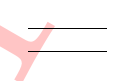
\begin{tikzpicture} \draw(0,0)--(1,0); \draw(0,0.3)--(1,0.3);\end{tikzpicture} &
        {\tikz[>=Stealth] \draw[->] (0,0) -- (1,0);} \\
        数据源或终点 & 数据处理 & 数据存储 & 数据流动 \\
    \end{tabular}
\end{table}

画DFD的方法:
\begin{enumerate}
    \item 确定系统的输入输出;
    \item \Point{由外向里}画顶层数据流图;
    \item 自顶向下逐层分解。
\end{enumerate}

实例:仓库订货系统、「口算高手」、客房管理系统(详见课件)。

\paragraph{数据字典(DD)}
\Concept{数据字典}(Data Dictionary)用来对数据流图的所有被命名的元素加以定义。它也是一种描述\Point{逻辑模型}的工具。

在数据字典中,我们会自顶向下地对一个字段的规则进行分解。常用规则:
\begin{itemize}
    \item $a+b$——由 $a$ 和 $b$ 构成;
    \item $[a|b]$——由 $a$ 或 $b$ 构成;
    \item $(a)$——元素 $a$ 出现零次或一次;
    \item $\{a\}$——元素 $a$ 出现零次或多次;
    \item $m\{a\}n$——元素 $a$ 出现 $m\sim n$ 次(当 $m=n$ 时即次数固定);
    \item $a\dots b$——取值为 $a\sim b$ 的任一个值;
    \item $"a"$——取值 $a$ 已经是最基本的,无需再度定义。
\end{itemize}

例如在学生—课程数据库中的数据字典可能的情况如下所示:

\begin{trivial}
    \begin{itemize}
        \item $\text{学号/Sno} = "2022" + 7\{\text{数字}\} 7$,$\text{数字} = "0"\dots "9"$
        \item $\text{姓名/Sname} = \Big[2\{\text{汉字}\}6 \Big| 1\{\text{汉字}\} 8 + "\text{·}" + 1\{\text{汉字}\} 8\Big]$ \textcolor{gray}{\small(考虑少数民族名)}
        \item $\text{性别/Ssex} = ["\text{男}"|"\text{女}"]$
        \item $\text{成绩/Grade} = "0"\dots "100"$
    \end{itemize}
\end{trivial}

\subsection{成本/效益分析}
\Concept{成本/效益分析}是为了从经济角度评估开发一个新项目的可行性。

成本估计一般用代码行技术、任务分解技术。

效益估计一般用货币的时间价值、投资回收期、纯投入等。

可行性报告参考格式:GB8567-88。

\section{软件定义·需求分析}
\begin{trivial}
    《原神》中的传奇工匠希诺宁,几乎什么工具都能打造。但对她来说,最难面对的客户是不知道自己想要的东西有多复杂的人。因此在开始打造以前,希诺宁总需要花费大量的精力帮助客户捋清需求。可见,需求分析是十分关键的一环。
\end{trivial}

\subsection{何为需求分析}
\Concept{需求分析}的目的是澄清客户需求,并把开发者和客户双方的理解表述成一份《软件需求规格说明书》。

\Concept{客户}包括提出要求、支付款项、选择、具体说明或使用软件产品的项目风险承担者(stakeholder)或是获得产品所产生结果的人。

需求分析的具体任务包括:
\begin{enumerate}
    \item 确定综合需求;
    \item 分析数据需求;
    \item 导出逻辑模型;
    \item 修正开发计划;
    \item 验证分析正确性;
    \item 编写需求说明书。
\end{enumerate}

软件的综合需求一般包括:
\begin{enumerate}
    \item \Point{功能}需求
    \item \Point{性能}需求
    \item \Point{可靠性可用性}需求
    \item 出错处理需求
    \item 接口需求
    \item \Point{约束}(环境约束、界面约束、用户因素约束、文档约束、数据约束、资源约束、安全保密要求约束、软件成本消耗与开发进度需求约束)
    \item 逆向需求
    \item 未来潜在需求
\end{enumerate}

需求获取的常见方法:
\begin{enumerate}
    \item 访谈
    \item 面向数据流自顶向下求精
    \item 应用规格说明
\end{enumerate}

需求分析实例:「口算高手」软件、远程路灯照明系统(详见课件)。

需求分析的四个阶段:
\begin{enumerate}
    \item \Point{调查研究}——需求调查,补充数据字典,修改IPO图
    \item \Point{分析与综合}——追踪数据流图,复查系统逻辑模型
    \item \Point{书写需求分析文档}——书写系统规格、数据要求、用户系统描述等文档
    \item \Point{需求分析评审}
\end{enumerate}

需求分析的步骤如图 \ref{fig:Demand_Analysis} 所示。
\begin{figure}[htb]
    \centering
    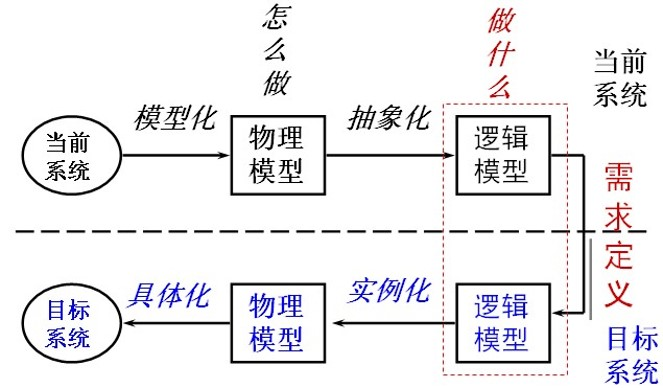
\includegraphics[width=8cm]{需求分析.jpg}
    \caption{需求分析的步骤}\label{fig:Demand_Analysis}
\end{figure}

需求分析阶段常用的逻辑模型:\Point{数据流图(DFD)}、\Point{E-R图}、类图、时序图、状态图、协作图等。

\subsection{结构化分析方法(SA)}
\Concept{结构化分析方法}(Structured Analysis)是一种面向数据流、自顶向下、逐步求精的方法。这种方法使用的建模工具有\Point{数据流图(DFD)}、\Point{数据字典(DD)}、结构化英语、判定表、判定树等。

\subsection{需求分析常用图形}
\paragraph{E-R图}
\Concept{实体—联系图},即 \Concept{E-R图},也就是「数据模型」\footnote{第四章课件的第三章回顾部分提到了,数据模型也称E-R模型。},是我们熟悉的一种概念模型,它是逻辑模型的一种。

E-R图的三要素:{\tikz\draw (0,0) rectangle (1,0.5);} \Point{实体对象}、{\tikz\draw (0,0) circle (0.3);} \Point{属性}、{\tikz\draw (-0.5,0)--(0,0.3)--(0.5,0)--(0,-0.3)--cycle;} \Point{联系}。

数据规范化用范式表示,分为1NF至5NF,其中1NF冗余程度最大,5NF冗余程度最小。

\paragraph{状态转换图}
\Concept{状态转换图}是描绘系统状态及其转换关系的图,它是逻辑模型的一种。这种图所包含的初始状态\Point{有且只有 1 个},终止状态有 0 个到多个,中间状态若干。我们在《数字逻辑》《编译原理》等课程已经见过状态转换图了。

其符号为:\raisebox{2pt}{\tikz\fill (0,0) circle (2pt);} 初态、{
\begin{tikzpicture}
                                            \fill (0,0) circle (2pt);
                                            \draw (0,0) circle (4pt);
                                          \end{tikzpicture}} 终态、
\raisebox{-3pt}{\tikz\draw[rounded corners=2pt] (0,0) rectangle (1,0.5);} 中间态。

\paragraph{层次方框图}
层次方框图是一种用树形结构描述数据层级结构的逻辑模型。

\paragraph{IPO图}
输入—处理—输出图,即\Concept{IPO图},是一种描述数据的输入、处理、输出关系的图形工具,同样属于逻辑模型。

\subsection{本章实例}
需求分析报告书写同样遵循自顶向下原则。参考 GB856T-88。

本章实例:考务处理系统(详见课件)。其绘制过程如下:
\begin{enumerate}
    \item 明确系统功能
    \item 绘制顶层数据流图(DFD):三个{\tikz\draw (0,0) rectangle (1,0.5);} 数据源和一个{\tikz\draw (0,0) circle (0.3);}数据处理枢纽。(从上数第一层)
    \item 细化 0 层数据流图。(从上数第二层)
    \item 细化 1 层数据流图。(从上数第三层)
\end{enumerate}

\section{软件开发·总体设计}
\subsection{设计过程}
\Concept{总体设计}也称为概要设计、初步设计,要考虑「怎么做」的问题。(上一章的需求分析考虑的是「做什么」的问题。)

总体设计的主要任务是:划分物理元素、确定软件结构。

总体设计两个阶段:\Point{系统设计}、\Point{结构设计}。

总体设计总共九个步骤:(其中 1--3 为系统设计)
\begin{enumerate}
    \item 设想供选择的方案;
    \item 选取合理的方案;
    \item 推荐最佳方案;
    \item 功能分解;
    \item 设计软件结构;
    \item 设计数据库;
    \item 制定测试计划;
    \item 书写文档;
    \item 检查和复审。
\end{enumerate}

\subsection{设计原理}
\paragraph{模块化}
\Concept{模块化设计}就是将大型软件划分成一个个小模块的设计方法。重要指导思想是功能分解、信息隐藏和模块独立性。

成本与模块的关系呈「V形」曲线,即合理的模块数目可以使成本最小化,过多或过少都不合适。

\paragraph{控制结构}
\Concept{控制结构}描绘了软件模块间的相连关系,用图结构表示。常见度量:
\begin{itemize}
    \item \Point{扇出}:一个模块直接调用的模块数(图的最大出度)
    \item \Point{扇入}:调用一个模块的上层模块数(图的最大入度)
    \item \Point{深度}:模块的层数(图的深度)
    \item \Point{宽度}:同一层的最大模块数
\end{itemize}

%例如课件中的例子,最多有 2 个模块调用了 \verb!Disp! 模块,因此扇入为 2;\verb!main! 模块直接调用的模块数最多,为 4 个,所以扇出为 4;体现在图中从上到下,\verb!main! 为第一层,\verb!Max_Value!、\verb!Min_Value!、\verb!Ave_Value! 为第二层,\verb!Disp! 为第三层,因此深度为 3;第二层的模块数最多,为
%
%Max_Value(array) { .Disp(Max_temp); }
%Min_Value(array) { .Disp(Min_temp); }
%Ave_Value(array) { }
%Disp(result_value) { }
%main() {
%    Max_Value(a[3][4]);
%    Min_Value(a[3][4]);
%    Ave_Value(a[3][4]);
%    Disp("The result is OK!");
%}

\paragraph{抽象} 抽象指反映本质特征而忽略细节。可能分为多层次抽象。

\paragraph{信息隐藏} 模块内部包含的信息,对于不需要这些信息的模块来说是不能访问的。

\paragraph{模块独立性} 以内聚与耦合定性度量模块独立性。

\subsubsection{耦合}
\Concept{耦合}用于衡量不同模块之间相互依赖的紧密程度,\Point{越低越好}。应该追求「松散耦合」的系统。从低耦合到高耦合的七种类型如下所示,示意图如图 \ref{fig:coupling} 所示。

\begin{enumerate}
    \item \Point{非直接耦合/无耦合}:两个模块没有直接关系,最低耦合。
    \item \Point{数据耦合}:两个模块传递的都是简单的数据,松散耦合。
    \item \Point{特征耦合/标记耦合}:两个模块传递的是数据结构(数组、记录等)或都与一个数据结构有关。特征耦合可以修改为数据耦合。
    \item \Point{控制耦合}:上层模块向下层模块传递的信息会控制下层模块的调用逻辑。去除控制耦合的好方法是,将下层模块的判定逻辑上移到上层模块中,「先判定再调用」;以及把下层模块分解。
    \item \Point{外部耦合}:模块与系统外部(I/O设备等)关联。外部耦合\Point{必不可少},但是数量应尽量少。
    \item \Point{公共耦合}:一组模块引用同一个公用数据区,如全局变量、共享内存等。这种耦合须慎用。
    \item \Point{内容耦合}:两个模块之间互相访问内部信息或代码重叠,或者一个模块多入口。这种耦合是最糟糕的。
\end{enumerate}

\begin{figure}[htb]
    \centering
    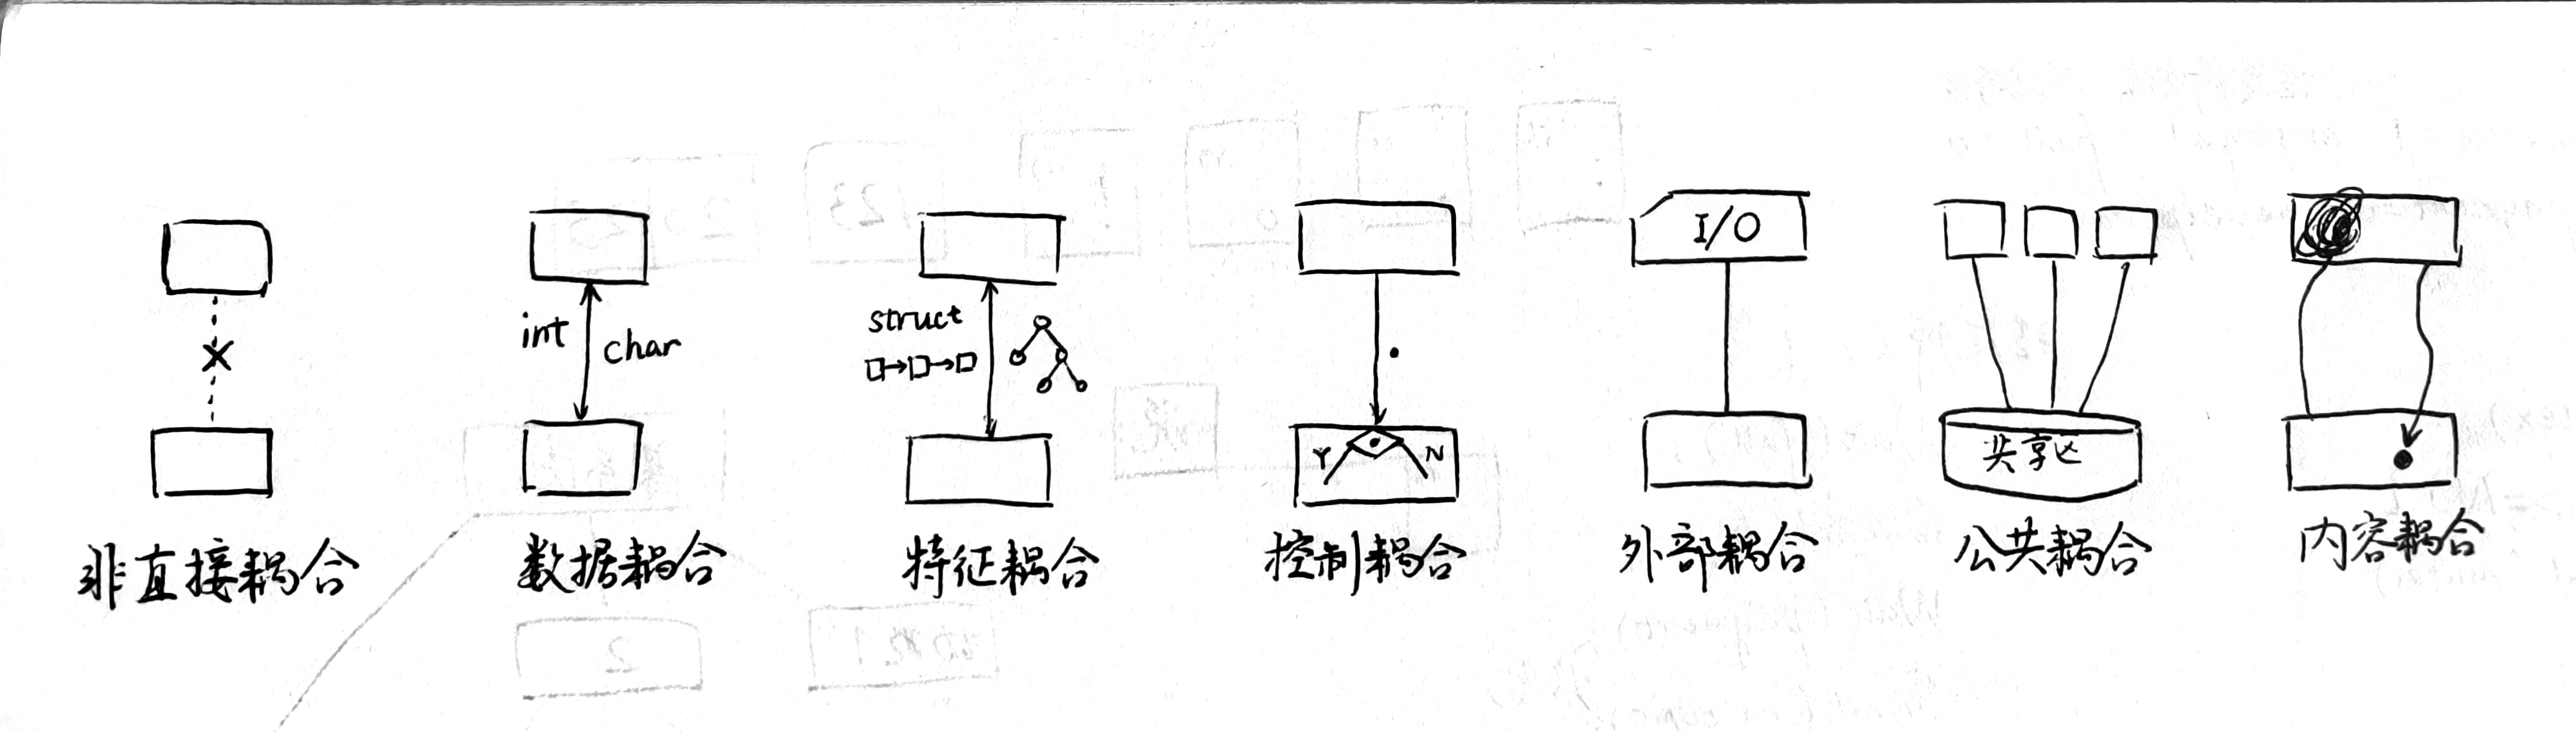
\includegraphics[width=\textwidth]{耦合.jpg}
    \caption{七种耦合类型示意图}\label{fig:coupling}
\end{figure}

耦合设计原则:
\begin{itemize}
    \item 多用数据耦合
    \item 少用控制耦合
    \item 限制公共耦合
    \item 避免内容耦合
\end{itemize}

\subsubsection{内聚}
\Concept{内聚}用于衡量一个模块内部各元素彼此结合的紧密程度,\Point{越高越好}。从低内聚到高内聚的七种类型如下:
\begin{enumerate}
    \item \Point{偶然内聚/巧合内聚}:模块内的语句没有任何联系。
    \item \Point{逻辑内聚}:将逻辑相似的功能组合在一个模块内。缺点是增加控制耦合,修改困难。
    \item \Point{时间内聚}:模块完成的功能必须在同一时间段内执行。
    \item \Point{过程内聚}:模块内各处理成分相关,且必须顺序执行。
    \item \Point{通信内聚}:模块内各部分使用相同的输入,或产生相同的输出。
    \item \Point{顺序内聚/信息内聚}:模块完成的功能都在同一数据结构上操作,且每个功能有唯一入口。
    \item \Point{功能内聚/理想内聚}:模块所有成分共同完成一个功能,缺一不可,也无冗余。最棒的内聚。
\end{enumerate}

\begin{trivial}
    笔者小记:判断何种「内聚」相当于是判断以什么理由将各个成分绑定在一个模块内。偶然内聚的理由根本没有,逻辑内聚的理由只是「看起来」逻辑相似,时间内聚的理由只是要在同一个时间段处理——这三者都属低内聚。过程内聚的理由是需要有先后关系,通信内聚的理由是需要处理同样的输入输出——这两者属于中内聚。顺序内聚的理由是操作对象数据结构相同,而功能内聚的理由即为实现的功能本身——这两种属于高内聚。
\end{trivial}

内聚设计原则:
\begin{itemize}
    \item 力求高内聚
    \item 可用中内聚
    \item 避免低内聚
\end{itemize}

\paragraph{内聚和耦合优先级}
实践表明,\Point{内聚}更重要些,高内聚意味着松耦合。

\subsection{启发规则}
常用的启发规则有:
\begin{enumerate}
    \item 提高模块独立性——提高内聚,降低耦合。
    \item 控制模块规模适中——过大则分解不充分,过小则接口复杂。
    \item 深度、宽度、扇入、扇出应适中。
    \item 模块的\Point{作用域在控制域之内}——保证模块可控。
    \item \textcolor{gray}{降低接口的复杂程度。}
    \item \textcolor{gray}{设计单入口、单出口模块。}
    \item \textcolor{gray}{模块功能应该可预测。}
\end{enumerate}

模块的\Concept{作用域}是指受该模块的一个判断所影响的模块之集合;\Concept{控制域}是指控制结构图中该模块本身与其子模块的集合,也就是「子树」。改变作用域和控制域方法:判断点上移,作用域对象下移。

\subsection{图形工具、面向数据流设计方法}
\paragraph{层次图}
\Concept{层次图}用于描绘软件的层次结构,矩形代表模块,连接代表调用关系。

\paragraph{HIPO图}
\Concept{HIPO图}就是「层次(Hierarchy)图 + 输入/处理/输出(IPO)图」的变种。相当于外层是层次图,每个模块加以编号;而内层即每个模块内部各有一个 IPO 图。

\paragraph{结构图(SC)}
\Concept{结构图}(Structure Chart)用于描绘模块间的信息传递关系,箭头表示调用关系,带注释的箭头表示传递的信息。层次图有传入、传出、变换、协调共四种模块,有选择调用和循环调用机制。

\paragraph{面向数据流设计方法}
数据流图分为「\Concept{变换型}」和「\Concept{事务型}」。变换型结构由输入、变换中心、输出三部分组成,而事务型结构由接受路径、事务中心、动作路径等组成。

变换型数据流图(DFD)经过变换分析可以得到结构图(SC)。事务型数据流图经过事务分析也可以得到结构图。

\paragraph{体系结构设计优化}
改进软件结构设计有 9 条原则。例如,消除重复功能,将作用域限制在控制域之内,模块大小适中等。

\section{软件开发·详细设计}
\Concept{详细设计}的目的是确定具体编程方案。

\subsection{结构程序设计}
\Concept{结构程序设计}采用自顶向下、逐步求精的设计方法和单入口、单出口的控制结构。

\begin{itemize}
    \item 经典结构程序设计:顺序、选择、循环。理论上最基本的控制结构为顺序和循环。
    \item 扩展结构程序设计:do-case(分支)、do-until
    \item 修正结构程序设计:break、continue、goto(少用)
\end{itemize}

\subsection{人机界面设计}
\Concept{人机界面设计}的 4 个设计问题:
\begin{enumerate}
    \item 系统响应时间
    \item 用户帮助设施
    \item 出错信息处理
    \item 命令交互
\end{enumerate}

人机界面设计指南:
\begin{enumerate}
    \item 一般交互指南
    \item 信息显示指南
    \item 数据输入指南
\end{enumerate}

\subsection{详细设计的工具}
详细设计的典型工具有:
\begin{itemize}
    \item \Point{程序流程图}
    \item \Point{盒图/N-S图}
    \item \Point{PAD图}(问题分析图)
    \item 结构化英语
    \item 判定表、判定树
    \item 过程设计语言(PDL)
\end{itemize}

其中盒图中的有些符号需要留意,如分支判断的结果为假写在左边,为真写在右边;直到型循环和当型循环的折角方向也不一样。

判定表由四部分组成:条件桩、操作桩、条件条目、操作条目。

可能需要掌握例子如一元二次方程求解过程的程序流程图、盒图画法。

\section{软件开发·编码}
\begin{trivial}
    由于课件的原型不晚于2010年,大约在2003年前后,因此课件内举的一些例子(如程序设计语言)略显陈旧。
\end{trivial}

\Concept{编码}就是用程序设计语言书写程序。

程序设计语言可分为机器语言、汇编语言、高级语言、第四代语言。

选择语言要求:用户要求、编译程序要求、软件工具要求、工程规模要求、程序员知识、可移植性、应用领域等。

编码风格规则:程序内部的文档、数据说明、语句构造、输入输出、效率等。

\section{软件开发与维护·测试}
\Concept{测试}是为了发现程序中的错误而执行程序的过程。然而测试成功并不能证明程序一定没有 bug。

测试的基本步骤:模块测试、子系统测试、系统测试、验收测试、平行运行。

\subsection{单元测试}
\Concept{单元测试}用详细设计描述作为指南,对重要的数据通路进行测试。可以使用\Point{白盒测试}法。

单元测试的重点:
\begin{itemize}
    \item 模块接口调试
    \item 局部数据结构测试
    \item 重要的执行通路测试
    \item 出错处理通路测试
    \item 边界条件测试\textcolor{gray}{(参加过CSP考试的应该深有体会)}
\end{itemize}

\subsection{集成测试与确认测试}
\Concept{集成测试}是指测试和组装软件的系统化技术,主要目标是发现与\Point{接口}相关的问题。两种方法:非渐增式测试、渐增式测试。两种结合方式:自顶向下结合、自底向上结合。

假设有 4 个模块,分别编号为 1,2,3,4,那么两种方法的测试流程可能如下:
\begin{itemize}
    \item 非渐增式测试:分别测试 1, 2, 3, 4, 1234。
    \item 渐增式测试:分别测试 1, 12, 123, 1234。
\end{itemize}

\Concept{确认测试}也称\Concept{验收测试},是为了检测软件的有效性。一般使用\Point{黑盒测试}法。在需求分析阶段产生的文档是软件有效的标准,也是验收测试的基础。

以某游戏的 Alpha 和 Beta 测试为例:
\begin{itemize}
    \item Alpha 测试:也称「内测」,环境相对封闭,通常是公司内部工作人员参与,对外界保密。
    \item Beta 测试:也称「公测」,环境相对开放,通常需要一些玩家的游玩体验与反馈意见。
\end{itemize}

\subsection{白盒测试与黑盒测试}
\paragraph{白盒测试}
\Concept{白盒测试}也称\Concept{结构测试},主要用于检测软件编码过程中的错误,用于前期测试。

白盒测试的测试用例设计,采用\Point{逻辑覆盖法},由弱到强的偏序关系分为:
\begin{enumerate}
    \item \Point{语句覆盖}:每条语句至少执行一次。
    \item \Point{判定覆盖/分支覆盖}:每次判定的真假分支至少执行一次。
    \item \Point{条件覆盖}:每次判定的每个条件的可能取值至少执行一次。例如,对 $(x>3) \mathrm{AND} (y<2)?$ 的条件,测试用例至少要包括 $x>3$、$x\leqslant 3$、$y<2$、$y\geqslant 2$ 的取值。
    \item \Point{判定—条件覆盖}:判定覆盖 + 条件覆盖。
    \item \Point{条件组合覆盖}:每个判定表达式的各种可能组合至少出现一次。
    \item 点覆盖、边覆盖、路径覆盖:至少经过流图的每个点/边/路径一次。
\end{enumerate}

\paragraph{黑盒测试}
\Concept{黑盒测试}也称\Concept{功能测试},主要检测软件的每一个功能是否能够正常使用,用于后期测试。

划分「等价类」的几条启发式规则,这里用形式化定义表述,请结合课件观看:
\begin{enumerate}
    \item 规定输入值范围为连续值 $[x,y]$,假设输入值为 $I$,则划分出三个等价类:
    \begin{itemize}
        \item 有效等价类:$I\in[x,y]$;
        \item 无效等价类:$I\in(-\infty,x)$、$I\in(y,\infty)$。
    \end{itemize}
    \item 规定输入数据个数 $a[0]\sim a[x]$,假设测试的下标为 $I$,则划分出三个等价类:
    \begin{itemize}
        \item 有效等价类:$I\in [0,x)$
        \item 无效等价类:$I\in (-\infty,0)$、$I\in [x,\infty)$
    \end{itemize}
    \item 规定输入值范围为离散值 $A=\{a_1,a_2,\dots, a_n\}$,假设输入值为 $I$,则划分出两个等价类:
    \begin{itemize}
        \item 有效等价类:$I\in A$
        \item 无效等价类:$I\notin A$
    \end{itemize}
    \item 规定输入值的数据类型或规则 $r_0$,假设输入数据的数据类型或规则满足 $I$,则划分出若干个等价类:
    \begin{itemize}
        \item 有效等价类:$I = r_0$
        \item 无效等价类:$I = r_1, r_2, r_3\dots$(总之 $I\ne r_0$)
    \end{itemize}
    \item 规定输入值范围为连续值 $[x,y]$,其中 $x<0$,$y>0$,假设输入值为 $I$,则划分为五个等价类:
    \begin{itemize}
        \item 有效等价类:$I\in [x,0)$、$I = \{0\}$、$I \in (0,y]$
        \item 无效等价类:$I\in(-\infty,x)$、$I\in(y,\infty)$。
    \end{itemize}
\end{enumerate}
总的来说,无效等价类就是有效等价类的补集。

在黑盒测试中,需要为有效等价类设计测试用例,还需要为每个无效等价类分别设计测试用例,因此理论上最少测试用例数量 = 无效等价类数量 + 1。

\section{软件维护·维护}
软件\Concept{维护}是指为了改正错误(bug)或满足新的需要而修改软件的过程。

维护的种类:
\begin{itemize}
    \item \Point{纠错性/改正性}维护——例如修正一个在开发阶段已发现的 bug
    \item \Point{适应性}维护——例如本来在 Win10 操作系统下运行的软件,开发 Win11 的 API
    \item \Point{完善性}维护——例如电商平台改进搜索算法,使结果更贴合用户意图
    \item \Point{预防性}维护——例如对老旧项目代码进行重构(如更新依赖库)
\end{itemize}

\begin{quote}\small\color{gray!50!black}
    【小测试】以下是游戏《原神》5.5 版本「众火溯还之日」更新公告节录,请对以下每一条更新判别分类:
\begin{enumerate}
    \item 「纳塔」地区开放新地图「安饶之野」「远古圣山」——???
    \item 修复了角色「绮梦缱绻·梦见月瑞希(风)」施放下落攻击后,武器显示异常的问题——???
    \item 「神瞳共鸣石」成功寻找到神瞳后的冷却时间由5分钟调整为2分钟——???
    \item 增加了对iPad Air (M3) 和iPad (A16)设备的适配支持——???
\end{enumerate}
答:1.完善性维护;2.纠错性维护;3.完善性维护;4.适应性维护
\end{quote}


软件维护的特点:结构化维护和非结构化维护差别巨大、维护代价高昂、维护的问题很多等。

决定软件可维护性的因素:可理解性、可测试性、可修改性、可移植性、可重用性。

\section{面向对象方法学}
\subsection{何为面向对象方法学}
在\Concept{面向对象方法学}中,任何事物都是对象,对象分解取代了功能分解。

面向对象方法学的要点(总结为一个等式):
\begin{equation}\label{eq:OO}
    \Point{\text{面向对象} = \text{对象} + \text{类} + \text{继承} + \text{消息}}
\end{equation}

面向对象方法学的优点:
\begin{itemize}
    \item 与人类习惯的思维方式一致
    \item 稳定性好
    \item 可重用性好
    \item 较易开发大型软件产品
    \item 可维护性好
\end{itemize}

\paragraph{相关概念}
类与对象的基本认识:
\begin{itemize}
    \item \Concept{对象}是对某个实体的抽象,形式化定义为 $\langle\text{对象名},\text{操作},\text{数据结构},\text{受理消息}\rangle$。其特点是:
    \begin{trivial}
        以数据为中心、对象是主动的、实现的数据封装、本质上具有并行性、模块独立性好。
    \end{trivial}
    \item \Concept{类}是对相同属性和行为的一个或多个对象的描述。
    \item \Concept{实例}是某个特定的类描述的一个具体的对象。
    \item \Concept{消息}是对象间交互的核心机制。通过消息,对象可以请求其他对象执行特定操作。一个消息通常由三部分组成:\Point{接收对象}、\Point{方法名}、\Point{参数列表}。
    \item \Concept{方法}是对象所能执行的操作。在C++中,「方法」也叫做「成员函数」。
    \item \Concept{属性}是类中所定义的数据项。
\end{itemize}

面向对象的三大特征:继承性、封装性、多态性。
\begin{itemize}
    \item \Concept{封装}是指把数据和方法集中放置于对象的内部。
    \item \Concept{继承}是指子类能够获得父类的一些已有性质和特征。
    \item \Concept{多态}是指允许对象以多种形式出现。
\end{itemize}

多态性似乎有些难以理解,举个例子:
\begin{lstlisting}[language=Java]
public class Main{
    void show(int i){
        System.out.println("Integer: " + i); //输出语句
    }
    void show(double d){
        System.out.println("Double: " + d);
    }
    void show(String s){
        System.out.println("String: " + s);
    }
}
\end{lstlisting}
这个 Java 代码块的 Main 类的 show 方法允许接收不同类型的参数,这就体现了多态性,同时也是函数重载的一个例子。

\Concept{重载}是实现多态性的保证,其主要分为两种类型:
\begin{itemize}
    \item 函数重载:同一个函数名可以有不同的参数列表;
    \item 运算符重载:允许用户重定义既有运算符的行为。
\end{itemize}

采用\Concept{面向对象建模}开发软件,通常需要建立以下三种模型:
\begin{enumerate}
    \item \Point{对象模型}——描述系统数据结构
    \item \Point{动态模型}——描述系统控制结构
    \item \Point{功能模型}——描述系统功能
\end{enumerate}

这三种模型的关系:相互补充,相互配合。(课件9.7小节)
\begin{enumerate}
    \item 对象模型——定义了做事情的实体
    \item 动态模型——规定了什么时候做事情
    \item 功能模型——指明了系统应该做什么
\end{enumerate}

\subsection{对象模型}
\Concept{对象模型}是对对象及其关系的映射,描述了系统的静态结构。通常使用统一建模语言(UML)的\Point{类图}来建立对象模型。

类图的基本符号,从上到下共三层,如表 \ref{tab:UML-class} 所示。

\begin{table}[htb]
    \centering
    \begin{minipage}[c]{.49\textwidth}
        \centering
        \vspace{0pt}
        \begin{tabular}{|c|}
        \hline
            类名 \\
        \hline  
            属性 \\
        \hline
            方法 \\
        \hline
        \end{tabular}
        \subcaption{类图的基本符号}
    \end{minipage}
    \begin{minipage}[c]{.49\textwidth}
        \centering
        \vspace{0pt}
        \begin{tabular}{|ll|}
        \hline
            & 宠物 \\
        \hline
            \verb!+! & 名字: String \\
            \verb!#! & 年龄: Integer = 0 \\
        \hline
            \verb!+! & 吃(食物) \\
            \verb!+! & 睡() \\
            \verb!-! & 玩耍() \\
        \hline
        \end{tabular}
        \subcaption{类图举例}
    \end{minipage}
    \caption{UML 类图的画法}\label{tab:UML-class}
\end{table}

其中前面可能冠以符号代表可见性:\verb!+! 代表 public,\verb!-! 代表 private,\verb!#! 代表 protected。

类与类之间可能存在的关系,如表 \ref{tab:class_relationship} 所示。

\begin{table}[htb]
    \centering\small\hspace*{-2em}
    \begin{tabular}{ccccc}
    \toprule
        关系类型 & 强度 & 生命周期依赖 & 举例(UML 画法) & 解释\\
    \midrule
        \Point{泛化/继承} & 最强 & 子类继承父类 &
            {\tikz\draw[->, >={Latex[open]}] (0,0)node[left]{狗}--(0.5,0)node[right]{动物};}
            & 狗「是一种(is-a)」动物 \\
        \textcolor{gray}{组合} & 强 & 部分随整体销毁 &
            {\tikz\draw[<-, >={Diamond}] (0,0)node[left]{窗口}--(0.5,0)node[right]{菜单};}
            & 窗口销毁时菜单也不存在 \\
        \Point{聚合/聚集} & 中 & 整体部分关系 &
            {\tikz\draw[<-, >={Diamond[open]}] (0,0)node[left]{教室}--(0.5,0)node[right]{学生};}
            & 学生独立于教室存在 \\
        \Point{关联} & 弱 & 语义上有关系 &
            {\tikz\draw  (0,0)node[left]{教师}--(0.5,0)node[right]{课程};}
            & 教师与课程长期关联 \\
        \Point{依赖} & 最弱 & 临时使用 &
            {\tikz\draw[->, dashed, >={Latex}]  (0,0)node[left]{报告生成器}--(0.5,0)node[right]{数据};}
            & 报告生成器类临时依赖数据类\\
        \textcolor{gray}{细化} & 最弱 & 描述层次更细 & 
            {\tikz\draw[->, dashed, >={Latex[open]}]  (0,0)node[left]{设计类}--(0.5,0)node[right]{分析类};}
            & 设计类在分析类基础上详细描述 \\
    \bottomrule
    \end{tabular}
    \caption{类与类的关系表}\label{tab:class_relationship}
\end{table}
需要指出的是,聚合是一种特殊的关联,组合是一种特殊的聚合。

此外对于关联关系,我们可能会在箭头的两端写上重数:
\begin{itemize}
    \item $0\dots 1$ —— 表示零个或一个
    \item $0\dots *$ 或 $*$ —— 表示零个或多个
    \item $1\dots *$ 或 $1+$ —— 表示一个或多个
    \item $n$ —— 表示 $n$ 个
    \item $m\dots n$ —— 表示 $m$ 个到 $n$ 个
\end{itemize}
例如,一个作家使用一台或多台计算机,而一个计算机被零个或多个作家使用。

\begin{quote}\small\color{gray!50!black}
    【小测试】在横线内填写合适的关系。备选:A.关联;B.聚合;C.泛化;D.实现;E.依赖
\begin{enumerate}
    \item 在图书管理系统中,读者包含教工和学生,其中教工可以借 10 本书,本科生可以借 6 本书,则本科生和书之间是\uline{\qquad}关系,读者和本科生是\uline{\qquad}关系。
    \item 交通工具与卡车之间是\uline{\qquad}关系,卡车与发动机之间是\uline{\qquad}关系。
    \item 公司与部门之间是\uline{\qquad}关系。
    \item 人借助船渡河,人与船之间是\uline{\qquad}关系。
\end{enumerate}
答:1. A.关联、C.泛化;2. C.泛化、B.聚合(或组合聚集);3. B.聚合;4. E.依赖
\end{quote}

%\begin{enumerate}
%    \item \Point{关联}——两个类的对象之间存在语义上的联系。
%    \item \Point{聚集/聚合}——关联的特例,表示类与类之间是整体和部分的关系。
%    \item \Point{泛化/继承}——is-a关系,子类继承父类。
%    \item \Point{依赖和细化}——前者指一种影响关系,后者指更详细地描述。
%    \item \textcolor{gray}{实现——指定两个实体间的一个合同,一个实体定义一个合同,而另一个实体保证履行该合同。}
%\end{enumerate}

\subsection{动态模型、功能模型}
\Concept{动态模型}是一种特别的\Point{状态图},描述对象在其生命周期的各种状态,以及状态之间的转换关系。

\Concept{功能模型}直接反映用户对目标系统的要求,由一组\Point{数据流图}(DFD)或者 UML 中的\Point{用例图}组成。以用例图建立的功能模型,也叫做\Concept{用例模型}。一幅用例图所包含的模型元素有:系统、行为者、用例及用例之间的关系。

\section{统一建模语言(UML)}
\Concept{统一建模语言}(Unified Modeling Language)是一个通用的可视化建模语言,是用于对软件进行描述、可视化处理、构造和建立软件系统支配的文档。

UML 包含 5 种视图:
\begin{trivial}
    用例视图、逻辑视图、组件视图、实现视图、部署视图
\end{trivial}

课件给出的 UML 的图例:
\begin{itemize}
    \item 用例图
    \item 活动图
    \item 顺序图
    \item 协作图
    \item 类图
    \item 状态图
    \item 组件图
    \item 部署图
\end{itemize}

\newpage
\backgroundsetup{contents=
\includegraphics{下半示例.png}, center, scale=1, angle=0, opacity=1}
\BgThispage
\printindex

\end{document} 